%!TEX TS-program = xelatex
\documentclass[12pt, a4paper, oneside]{article}

\input{preamble.tex}

\begin{document}

\section*{Quiz 5: рекуррентные нейронные сети}

\epigraph{Боже! Моё паучье чутьё просто сходит с ума!}{\textit{Питер Паркер}}

\vspace{-0.5cm}
\subsection*{[7] Задание 1}
\vspace{-0.5cm}

У Шмидхубера есть рекуррентная  ячейка, которая описывается следующими уравнениями 

\begin{equation*} 
	\begin{aligned}
	c'_t &= \phi_c(W_c x_t + V_c h_{t-1} + b_c) \\
	i_t &= \phi_i(W_i x_t + V_i h_{t-1} + b_i) \\
	f_t &= \phi_f(W_f x_t + V_f h_{t-1} + b_f) \\
    o_t &= \phi_o(W_o x_t + V_o h_{t-1} + b_o) \\
    c_t &= f_t \odot c_{t-1} + i_t \odot c'_t \\
    h_t &= o_t \odot \phi_h(c_t) \\
    y_t &= \phi_y(U\cdot c_t + b_y)
	\end{aligned}
\end{equation*} 

Изобразите эту ячейку в виде вычислительного графа. Кратко поясните смысл каждого уравнения. Укажите конкретные функции активации, которые бы вы взяли вместо $\phi_c, \phi_i, \phi_f, \phi_o, \phi_y$ Почему вы выбрали именно такие функции? 

Под операцией $\odot$ подразумевается поэлементное умножение. Под операцией $\cdot$ матричное умножение.

\vspace{-0.5cm}
\subsection*{[3] Задание 2}
\vspace{-0.5cm}

Щмидхуберу кажется, что следующий мем очень смешной. Объясните, почему Шмидхубер так думает.

\begin{center} 
    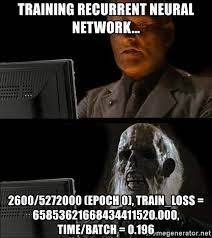
\includegraphics[scale=0.9]{rnn-memes.jpeg} 
\end{center}

\end{document}